% !TeX spellcheck = pl_PL
\chapter{Uwagi o przebiegu i wynikach prac}
W końcowej wersji aplikacji udało się spełnić wszystkie wymagania opisane w \ref{chap:wymagania}: tworzenie sieci przepływowych, ich serializację oraz algorytmy wyszukiwania maksymalnego przepływu. Wszystkie funkcjonalności zostało wielokrotnie przetestowane, chociaż bez testów automatycznych.
\section{Nowe technologie}
Język C++ został poznany w toku studiów, jednak platforma Qt, która została wybrana w rozdziale \ref{ssec:technologieJezyk} jako wykorzysta platforma graficzna, nie znajdowała się w programie studiów inżynierskich. Musiano poświęcić dużo dodatkowego czasu na samo zapoznanie się z technologią, w szczególności zrozumienie działania \textit{sygnałów} i \textit{slotów} jako podstawowej metody komunikacji pomiędzy widżetami. Dodatkowej pracy wymagało ponadto zsynchronizowanie platformy Qt z Visual Studio poprzez dodatek. Aby było to możliwe należało pobrać cały kod źródłowy Qt (poprzez konsolę Git i skrypty napisane w Perl) na lokalny dysk i zbudować całość kompilatorem jaki był wykorzystany w trakcie pracy (MSVC v12.0 x64). Tylko w tak skompilowanym Qt można było tworzyć programy i debugować je w Visual Studio.\\\indent
W trakcie pracy nad aplikacją wielokrotnie pojawiała się potrzeba bądź chęć skorzystania z gotowych bibliotek do wykonania pewnych funkcjonalności, m.in. parsowanie plików XML opisane w \ref{sec:serializacja}. Ponadto w aplikacji wykorzystano niektóre możliwości zbioru bibliotek \textbf{\textit{Boost}}, m.in. bibliotekę \emph{lexical\_cast}, która umożliwiała wygodną i bardzo bezpieczną konwersję elementarnych typów danych. Wykorzystano również bibliotekę \textbf{\textit{libconfig}}, której możliwości i czytelny format plików wejściowych wykorzystano do stworzenia prostego pliku konfiguracyjnego całej aplikacji. Jednak w przeciwieństwie do bibliotek Boost, libconfig był dołączany dynamicznie i skompilowana biblioteka DLL musi być dołączona do wersji \textit{release} aplikacji.
\section{Zachowanie zasad SOLID}\label{sec:solid}
Aplikacja była pisana z myślą o potencjalnych zmianach i rozszerzeniach, jakie mogą w niej zajść. W trakcie pracy nad rozwojem aplikacji starano się przestrzegać pięciu zasad określonych przez koncept SOLID \cite{id:CleanCodeSolid}\cite{id:solidWebsite}, ponieważ największymi problemami napotkanymi w czasie pracy były te związane z zaprojektowaniem aplikacji. Jaką strukturę powinna mieć sieć przepływowa, jak rozdzielić logikę od reprezentacji, jakie wzorce projektowe zastosować itp.
\subsection{Zasada \textit{Single responsibility}}
Pracując nad podstawową strukturą sieci przepływowej, jaka będzie wykorzystywana w całej aplikacji, starano się wprowadzić rozdzielenie grafu wyłącznie logicznego (\emph{Graph}) oraz jego reprezentacji w polu edycyjnym Qt (\emph{GraphImage} : \emph{QGraphicsItem}). Klasa reprezentacji zawiera wskaźnik do swojej struktury logicznej na podstawie której jest budowany rysunek w Qt.
\begin{figure}[H]
	\centering
	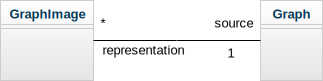
\includegraphics[width=0.4\linewidth]{./img/SOLID_SR.pdf}
	\caption{Rozdzielenie rysunku i logiki}
	\label{fig:SOLD_SR}
\end{figure}
Jednakże wierzchołki i łuki również potrzebowały dodatkowych informacji o ich sposobie rysowania, m.in. pozycji, wielkości i kolorów, więc dla reprezentacji ich graficznej również powstały dodatkowe klase (\emph{VertexImage}, \emph{EdgeImage}). Wadą tego rozwiązania było powielenie informacji, de facto w programie istniały dwie reprezentacje połączeń wierzchołków i krawędzi. Klasy z sufiksem \emph{Image} dziedziczą po \emph{QGraphicsItem} z platformy Qt, były więc wymagane do poprawnego wyświetlenia struktur graficznych. W tym przypadku klas pierwotnych, \emph{Graph}, \emph{Vertex} oraz \emph{Edge}, mogłoby nie być, a struktura grafu zawarta w \emph{GraphImage} być jedyną strukturą tworzącą graf. Jednak na tym etapie rozwoju koszt refaktoryzacji był większy niż płynące z niej korzyści, więc zależność między logiką, a reprezentacją pozostała niezmieniona.
\subsection{Zasada \textit{Open / closed}}
W pracy zostały zrealizowane jedynie sieci przepływowe, które są tylko jednym z wielu rodzajów grafów. Aplikacja była pisana z myślą, że w przyszłości może zostać rozszerzona do prezentacji innych algorytmów, na innych strukturach grafowych. Dlatego została utworzona klasa nadrzędna \emph{GraphImage} reprezentująca każdy typ grafu. Elastyczną rozszerzalność starano się zapewnić wykorzystując wzorce projektowe. O tym, czy graf jest ważony (posiada funkcję odwzorowująca jego zbiór krawędzi w zbiór liczb), decyduje odpowiedni obiekt klasy \textbf{\textit{strategii}} \cite{id:WzorceProjektoweStrategia}, który jest wstrzykiwany do grafu. Sieć przepływowa zawsze posiada strategię grafu ważonego. Zbiór narzędzi do edycji grafu, który przedstawia pasek narzędziowy, został oparty o wzorzec \textbf{\textit{stanu}} \cite{id:WzorceProjektoweStan}. Z punktu widzenia klas zewnętrznych narzędzie jest tylko jedno, pod wpływem naciśnięcia przycisku zmienia ono tylko swój stan wewnętrzny. Dzięki temu, aby dodać kolejne narzędzie, nie trzeba modyfikować istniejącego kodu, wystarczy jedynie utworzyć nową klasę - funkcjonalność jest odporna na zmiany, otwarta na rozszerzenia. Każda klasa narzędzia jest \textbf{\textit{singletonem}} \cite{id:WzorceCppSingleton}, w całej aplikacji potrzebne są wyłącznie pojedyncze egzemplarze. Lista algorytmów, jaka wyświetlana jest w okienku \textit{"Dostępne algorytmy"}, oparta  jest o \textbf{\textit{fabrykę obiektów}}. Klasy algorytmów do wyszukiwania maksymalnego przepływu same się w niej rejestrują przy uruchomieniu programu (\cite{id:WzorceCppFabryka}), a przy wybraniu jednego z nich jest pobierany wskaźnik do metody fabrykującej, która tworzy użytkowany obiekt algorytmu. W konsekwencji tego dodanie kolejnego algorytmu wymaga jedynie utworzenia nowej klasy. Fabryka również jest singletonem, potrzeba tylko jednej utworzonej na początku pracy aplikacji.
\subsection{Zasada \textit{Liskov substitution}}
Hierarchia dziedziczenia w aplikacji nie jest duża, ale zdarzały się momenty, kiedy i ta zasada była łamana. Konstruktor reprezentacji grafu otrzymuje jako parametr wskaźnik na konfigurację grafu.
\begin{minted}
[
frame=lines,
framesep=2mm,
]{cpp}
explicit GraphImage(GraphConfig * config);
\end{minted}
Tworząc konstruktor sieci przepływowej (klasa \emph{FlowNetwork}), dziedziczącej po grafie, w zamierzeniu miał on otrzymywać jeszcze informację, który wierzchołek ma być źródłem, a który ujściem.
\begin{minted}
[
frame=lines,
framesep=2mm,
]{cpp}
explicit FlowNetwork(GraphConfig * config, int source, int target);
\end{minted}
Jednak takie podejście uniemożliwiało utworzenia obiektu sieci przepływowej w ten sam sposób, co grafu, i należało w każdej metodzie, która sieć tworzyła, przekazywać owe dwa dodatkowe parametry. Co więcej, z czasem informacja o źródle i ujściu okazywała się zbędna. Każdy graf tworzony od nowa jest pusty i dopiero użytkownik aplikacji, w czasie budowy sieci, decyduje, który wierzchołek ma być źródłem, a który ujściem. Były potrzebne do tego dwie nowe metody, a nie parametry konstruktora.
\subsection{Zasada \textit{Interface segregation}}
Innym problemem było wyznaczenie poprawnych interfejsów do obsługi algorytmów wyszukiwania maksymalnego przepływu. Po przeczytaniu analizy algorytmów wydawało się, że dla każdego algorytmu wystarczą trzy abstrakcyjne funkcje: utworzenie sieci residualnej, znalezienie przepływu w tej sieci i zwiększenie przepływu w sieci pierwotnej, które będą wykonywane w pętli, aż do znalezienia maksymalnego przepływu. Algorytm Forda-Fulkersona idealnie wpisywał się w ten schemat, ale algorytmy Dinica i Mkm wymagały pewnych zmian. Po pierwsze, potrzebowały warstwowej sieci residualnej, ale tu wystarczyło tylko zmienić treść funkcji, a algorytm tworzenia warstwowej sieci wydzielić do wspólnej klasy. Po drugie, wymagały utworzenia przepływu blokującego zamiast ścieżki powiększającej i tu również, z punktu widzenia logiki, wystarczyłoby przeciążenie funkcji do znajdowania przepływu w sieci residualnej. Jednak tworzenie przepływu blokującego jest procesem o wiele bardziej skomplikowanym niż znalezienie ścieżki powiększającej i aby aplikacja mogła spełnić swój walor edukacyjny, on również powinien zostać zilustrowany. Zrodziła się potrzeba, aby algorytmy Dinica i MKM posiadały dwie dodatkowe funkcje: tworzenie przepływu blokującego i zwiększenie przepływu w nim. Działanie algorytm było przedstawiane w dedykowanym oknie i zależność wygląda następująco:
\begin{figure}[H]
	\centering
	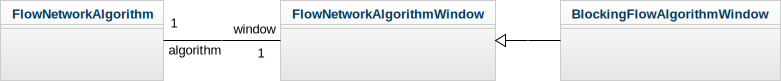
\includegraphics[width=0.8\linewidth]{./img/algWindowModel}
	\caption{Zależność między algorytmem, a oknem}
	\label{fig:algorytmOknoModel1}
\end{figure}
Okno z przepływem blokującym jedynie rozszerza funkcjonalność domyślnego okna dodając do niego podgląd zmian w owym przepływie. Jednak istniejąca do tej pory wersja okna posiadała obiekt algorytmu z interfejsem zawierającym trzy funkcje. Okno z przepływem blokującym również widziało tylko taki wskaźnik do algorytmu. Jeżeli okno potrzebowałoby dostępu do nowych funkcji, wymagane byłoby rzutowanie. Aby tego uniknąć model mógłby wyglądać następująco:
\begin{figure}[H]
	\centering
	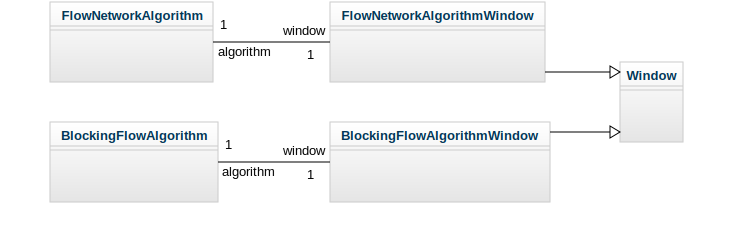
\includegraphics[width=0.8\linewidth]{./img/algWindowModel2}
	\caption{Zależność między algorytmami, a oknami}
	\label{fig:algorytmOknoModel2}
\end{figure}
Ale możliwe było podejście z wykorzystaniem wcześniejszego modelu (rys. \ref{fig:algorytmOknoModel1}). Tworzenie przepływu blokującego to wielokrotne szukanie ścieżek powiększających w warstwowej sieci residualnej, a zwiększenie przepływu w sieci pierwotnej polega na ich odwzorowaniu. Korzystając z pierwszego modelu można było zrealizować te dwie dodatkowe funkcje realizując już istniejące, wystarczyło jedynie zmieniać argumenty metod lub wywoływać je wielokrotnie. Odpowiadała za to klasa z oknem do przepływu blokującego. Dzięki temu kod stał się trochę mniej elastyczny i rozszerzalny, ale ilość pracy potrzebnej do zrealizowania tych dwóch algorytmów - znacznie mniejsza.
\subsection{Zasada \textit{Dependency inversion}}
Ta zasada nie była trudna do zachowania, chociaż nie była przestrzegana w całej aplikacji. Wszędzie, gdzie to było możliwe, klasy posiadały składowe, a metody argumenty, które były wskaźnikami lub referencjami na jak najogólniejsze struktury. Okno algorytmu posiada wskaźnik na abstrakcyjną klasę algorytmu, klasa związana ze stanem algorytmu zwraca wskaźnik na potrzebne okno, bez jawnego przekazywania informacji, czy to okno z przepływem blokującym lub nie, itp. Jeżeli zdarzały się klasy pochodne jako składowe lub argumenty, to dlatego, że były naprawdę wymagane, np. sieć przepływowa (klasa \emph{FlowNetwork}) dla algorytmów wyszukiwania maksymalnego przepływu lub tworzenia sieci residualnej. Hierarchia klas w aplikacji posiada kilka poziomów i na późnym etapie rozwoju aplikacji nie można było zrezygnować z dziedziczenia na rzecz pełnego \emph{DI} tak, by było to opłacalne.
\begin{figure}[H]
	\centering
	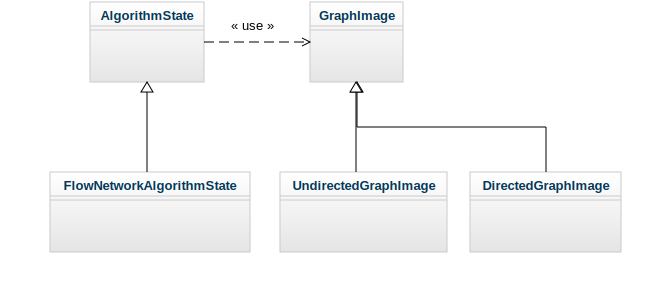
\includegraphics[width=0.8\linewidth]{./img/SOLD_DI.pdf}
	\caption{Przykład zastosowania zasady \textit{Dependency Inversion}}
	\label{fig:SOLD_DI}
\end{figure}
\section{Rozwój aplikacji}
Jak napisano w rozdziale \ref{ssec:kontrolaWersji} cały projekt z pracą inżynierską był założony na repozytorium kodu w serwisie \textit{Bitbucket}. Korzystając z wtyczki \textit{\textbf{Awesome Graphs for Bitbucket Server}} zostały utworzone grafy prezentujące postęp pracy inżynierskiej w postaci liczby zatwierdzonych zmian (ang. \emph{commits}) każdego dnia.
\begin{figure}[h]
	\centering
	\includegraphics[width=\textwidth]{./img/wykres1}
	\caption{Wygładzony wykres przedstawiający liczbę zmian w każdym tygodniu}
\end{figure}
\begin{figure}[h]
	\centering
	\includegraphics[width=\textwidth]{./img/wykres2}
	\caption{Zobrazowanie liczby zmian każdego dnia w postaci karty dziurkowanej}
\end{figure}